%! TEX root = ../main.tex

\chapter{Introduction}\label{chap:intro}

A recurring theme in statistics is that the quantity of scientific interest is not directly observable. Instead, one observes a transformed or corrupted version of it, and the task is to invert the transformation. In a \textit{statistical inverse problem}, the data $Z_1,\ldots,Z_n$ are drawn from a distribution $G_0$ that is linked to an unknown distribution $F_0$ through a forward operator $K$:
\[
G_0 = K(F_0).
\]
The goal is to recover $F_0$, or functionals thereof, from the observations. Problems of this form arise across a wide range of scientific disciplines. In astronomy, one cannot observe the full three-dimensional structure of a globular cluster --- a spherical aggregation of thousands of stars bound by gravity --- but only its two-dimensional projection on the sky. The apparent positions of stars are known functions of their true spatial positions, and recovering the three-dimensional radial distribution of stars from these projected observations requires inverting that geometric transform \cite{33,14}. In signal processing and epidemiology, a measured signal is the convolution of an unknown source distribution with a known noise kernel (arising when signal and noise are independent additive components), and deconvolution is required to recover the source \cite{84,83}. In causal inference from observational data, unobserved confounders create a systematic distortion between the observed data distribution and the causal distribution of interest; identifying and estimating the causal effect requires inverting this confounding mechanism \cite{120,205}. 

\begin{figure}[H]
\centering
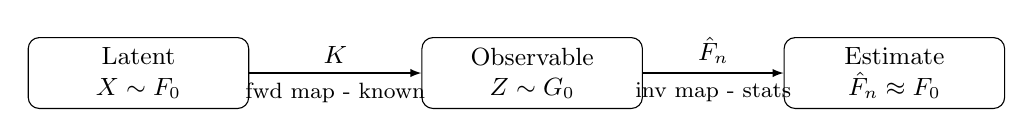
\begin{tikzpicture}[
  box/.style={draw, rounded corners, minimum width=2.8cm, minimum height=0.9cm,
              align=center, fill=white, font=\small},
  >=latex
]
  \node[box] (X) at (0,0)    {Latent\\$X \sim F_0$};
  \node[box] (Z) at (5,0)  {Observable\\$Z \sim G_0$};
  \node[box] (E) at (9.6,0)  {Estimate\\$\hat{F}_n \approx F_0$};

  \draw[->] (X) -- (Z) node[midway, above, font=\small] {$K$}
                        node[midway, below, font=\footnotesize] {fwd map - known};
  \draw[->] (Z) -- (E) node[midway, above, font=\small] {$\hat{F}_n$}
                        node[midway, below, font=\footnotesize] {inv map - stats};
\end{tikzpicture}
\caption{Schematic diagram of a statistical inverse problem. The forward operator $K$ maps the latent law $F_0$ to the observable law $G_0$. Statistical inference inverts this map from data $Z_1,\ldots,Z_n$. The thesis treats Wicksell's problem ($K$ = stereological transform, Chapters~2--3), nonparametric deconvolution ($K$ = convolution, Chapters~4), and proximal causal inference ($K$ = unobserved confounding mechanism, Chapter~5).}
\label{fig: inverse problem schematic}
\end{figure}

Despite their apparent diversity, these problems share a common mathematical skeleton: a known forward map $K$, an unknown object $F_0$, and noisy indirect observations (see Fig.\ \ref{fig: inverse problem schematic}), and they share thus a common set of statistical challenges.

\section{Statistical inverse problems and regularisation}\label{sec: inverse problems intro}
The fundamental difficulty of statistical inverse problems is their \textit{ill-posedness}: small perturbations in $G_0$ can correspond to large perturbations in $F_0$, because the operator $K$ typically smooths or compresses information. A classical illustration is deconvolution: in the frequency domain, $K$ multiplies by the characteristic function of the noise distribution, which may decay to zero. Inverting $K$ then amplifies high-frequency components, turning small noise into large estimation errors. As a consequence, unconstrained nonparametric estimators of $F_0$ tend to be erratic: non-monotone, irregular, or with infinite variance at rates too slow for statistical use and thus \textit{regularisation} is essential.

A natural and particularly powerful form of regularisation, which runs through this entire thesis, is the effective use of intrinsically present shape constraints. Distribution functions are monotone; their integral transforms inherit convexity or monotonicity properties; and estimators that respect these constraints are better conditioned. The analytical device used here is \textit{isotonisation}: replacing a naive unconstrained estimator by its projection onto the set of monotone functions, computed as the derivative of the least concave majorant of a primitive. This operation is computationally efficient (it reduces to the Pool-Adjacent-Violators Algorithm \cite{61}), tuning-parameter-free, and, in some cases, as established in this thesis, \textit{asymptotically efficient}.

\section{Efficiency and minimax lower bounds}\label{sec: efficiency intro}

A central question, once an estimator has been constructed, is whether it makes optimal use of the information in the data. The theory of statistical efficiency provides the language to answer this question precisely, and minimax theory provides lower bounds that characterise the fundamental difficulty of an estimation problem independently of any particular method. Let us start by briefly recalling efficiency in parametric models versus nonparametric models.

\paragraph{Efficiency.}
In a parametric model $\{P_\theta : \theta \in \Theta \subset \mathbb{R}^d\}$ with Fisher information matrix $I(\theta)$, the Cram\'{e}r--Rao inequality asserts that any unbiased estimator $T_n$ of $\theta$ satisfies $\mathrm{Var}_\theta(T_n) \geq I(\theta)^{-1}$, in the matrix sense. The classical asymptotic version, due to H\'{a}jek and Le Cam (cf.\ \cite{6}, Chapter~8), is sharper and more general: for any \textit{regular} estimator sequence $T_n$ of $\theta$, the limiting distribution $L$ in $\sqrt{n}(T_n - \theta) \to L$ must be a convolution $N(0, I(\theta)^{-1}) * M$ for some probability measure $M$. The Gaussian component $N(0, I(\theta)^{-1})$ cannot be removed; it is the irreducible cost of estimation, set by the Fisher information. An estimator is \textit{asymptotically efficient} if $L = N(0, I(\theta)^{-1})$, i.e.\ if $M = \delta_0$: there is no superfluous noise beyond what the data unavoidably carry. 

In a nonparametric model, where $F_0$ ranges over an infinite-dimensional class, there is no single Fisher information matrix. The relevant notion is instead the \textit{efficient asymptotic variance} for estimating a real-valued functional $T(F_0)$. Fix a smooth one-dimensional submodel $\{F_t\}$ passing through $F_0$ at $t=0$, differentiable in quadratic mean with score $h \in L^2_0(F_0)$. Suppose the functional $T$ is \textit{pathwise differentiable} at $F_0$ relative to such paths: the map $t \mapsto T(F_t)$ is differentiable at $t=0$, with derivative $\dot{T}_{F_0}(h)$ depending linearly and continuously on the score $h$. The Riesz representation theorem then gives a unique element $\tilde{\ell}_{F_0} \in L^2_0(F_0)$ --- the \textit{efficient influence function} --- such that $\dot{T}_{F_0}(h) = \langle \tilde{\ell}_{F_0}, h\rangle_{F_0}$ for all smooth directions $h$. The variance $\sigma^2_{\mathrm{eff}}(F_0) = \ex_{F_0}[\tilde{\ell}_{F_0}(Z)^2]$ is the \textit{semiparametric efficiency bound}: no regular estimator of $T(F_0)$ can have asymptotic variance smaller than $\sigma^2_{\mathrm{eff}}(F_0)$ (cf.\ \cite{13}, \cite{6}, Chapter~25). An estimator achieving this bound is \textit{semiparametrically efficient}. The bound is intrinsic: it depends only on $F_0$, the model and the functional $T$, not on the estimation method.

\paragraph{Minimax lower bounds.}
Efficiency bounds are local, attached to a fixed $F_0$. Minimax lower bounds certify that, over a class of distributions, no estimator can do better than a certain rate or variance; the class may be a fixed nonparametric family (a \textit{global} bound) or a shrinking neighbourhood of $F_0$ (a \textit{local} bound), and in general we allow it to depend on the sample size, writing $\mathcal{F}_n$. The prototypical statement is
\[
\liminf_{n\to\infty} \, \inf_{T_n} \, \sup_{F \in \mathcal{F}_n} \, r_n^2 \, \ex_{F}\!\big[\,T_n - T(F)\,\big]^2 \geq c > 0,
\]
for some sequence $r_n \to \infty$ and constant $c > 0$, where the infimum is over all estimator sequences. Taking $\mathcal{F}_n \equiv \mathcal{F}$ fixed gives a \textit{global} rate lower bound of order $r_n^{-1}$, uniformly over $\mathcal{F}$; taking $\mathcal{F}_n$ to shrink to $F_0$ at the appropriate rate gives a \textit{local asymptotic minimax} bound, which recovers the semiparametric efficiency bound of the previous paragraph as its sharp constant. This says that no estimator can estimate $T(F_0)$ at a rate faster than $r_n^{-1}$, uniformly over $\mathcal{F}$. The proof technique is typically a reduction to a hypothesis testing problem: if the estimation problem were easy, one could distinguish between hypotheses that are hard to separate, a contradiction. When an estimator $T_n$ satisfies $r_n(T_n - T(F_0)) \to N(0, \sigma^2(F_0))$ and $\sigma^2(F_0) = c$ matches the minimax lower bound, the estimator is simultaneously \textit{rate-optimal} and \textit{asymptotically efficient}: it is the best possible in both rate and constant.

A distinctive feature of inverse problems is that optimal estimation rates are often slower than the parametric $\sqrt{n}$. In Wicksell's problem, the optimal rate for estimating $F_0(x)$ is $\sqrt{n}/\sqrt{\log n}$, slower by a logarithmic factor. This logarithmic loss is a direct consequence of the ill-posedness of the Abel inversion: the operator $K$ loses information at a rate proportional to $(\log n)^{1/2}$, and this loss is irrecoverable. In deconvolution, rates can be polynomial in $n$ when the kernel is smooth \cite{84}. These non-standard rates mean that the classical $\sqrt{n}$-asymptotic theory does not apply directly; one must carry out the minimax analysis afresh for each problem.



\section[Uncertainty quantification and BvM theorem]{How UQ works in the frequentist versus Bayesian world}\label{sec: UQ intro}
A point estimator $\hat{F}_n(x)$ answers the question of where $F_0(x)$ likely is, but for scientific inference one also needs to know how reliably. We now give precise definitions of the two main tools for this.

A \textit{confidence set} at level $1-\alpha$ is a data-dependent set $C_n = C_n(Z_1,\ldots,Z_n)$ satisfying
\[
\inf_{F_0 \in \mathcal{F}} \pb_{F_0}\!\left(T(F_0) \in C_n\right) \geq 1-\alpha,
\]
for all $n$ (or asymptotically as $n\to\infty$), where $T(F_0)$ is the functional of interest and the infimum is over all $F_0$ in the model class $\mathcal{F}$. The probability is taken over the randomness in the data for fixed $F_0$: the set $C_n$ is random, and the parameter $T(F_0)$ is fixed. A $(1-\alpha)$ confidence set contains the true value in at least $1-\alpha$ of all hypothetical repetitions of the experiment.

Bayesian inference proceeds from a prior distribution $\Pi$ on the parameter $F$ and is based on the posterior distribution $\Pi\!\left(F \in \cdot \mid Z_1,\ldots,Z_n\right)$, the conditional distribution of the parameter given the data. A \textit{credible set} at level $1-\alpha$ is a set $D_n = D_n(Z_1,\ldots,Z_n)$ satisfying
\[
\Pi\!\left(F \in \mathcal{F} : T(F) \in D_n \mid Z_1,\ldots,Z_n\right) \geq 1-\alpha,
\]
Here the data are fixed and $F$ is random: the credible set concentrates $1-\alpha$ of the posterior mass on the event that the functional $T(F)$ takes a value in $D_n$. The Bernstein-von Mises (BvM) theorem is the classical result that connects these two objects in the parametric setting.

\paragraph{Building intuition: UQ in the parametric world.} Consider a parametric model $\{P_\theta : \theta \in \Theta \subset \mathbb{R}^d\}$ with Fisher information $I_\theta$ and a prior $\Pi$ that is absolutely continuous with a positive density near $\theta_0$. The BvM theorem (cf.\ \cite{6}, Chapter~10) states that the rescaled posterior distribution of $\sqrt{n}(\theta - \theta_0)$ converges in total variation to a Gaussian:
\[
\left\|\Pi\!\left(\sqrt{n}(\theta - \theta_0) \in \cdot \mid X_1,\ldots,X_n\right) - N\!\left(I_{\theta_0}^{-1}\Delta_{n,\theta_0},\, I_{\theta_0}^{-1}\right)\right\|_{\mathrm{TV}} \xrightarrow{P_{\theta_0}^n} 0,
\]
where $\Delta_{n,\theta_0} = n^{-1/2}\sum_{i=1}^n \dot\ell_{\theta_0}(X_i)$ is the rescaled score. The key consequences are: (i) the posterior concentrates at the rate $1/\sqrt{n}$, regardless of the prior; (ii) the asymptotic shape is Gaussian with variance $I_{\theta_0}^{-1}$, the Cramér--Rao bound --- so the posterior automatically concentrates at the rate and variance of an efficient estimator; (iii) the prior $\Pi$ disappears in the limit, meaning the result is robust to the choice of prior. Intuitively, the likelihood dominates the prior for large $n$, and the local shape of the likelihood is always approximately Gaussian around its maximum. For this reason, the BvM theorem is sometimes called the \textit{Bayesian central limit theorem}: just as the sample mean concentrates and Gaussianises by the CLT, the posterior concentrates and Gaussianises by the BvM. The practical upshot is that any $(1-\alpha)$ credible set is asymptotically a valid $(1-\alpha)$ frequentist confidence set, since both are determined by the same limiting Gaussian.

A useful reformulation, sometimes stated as a corollary, shifts the centring from $\theta_0$ to the maximum likelihood estimator $\hat\theta_n$. Under the same conditions, if $\hat\theta_n$ satisfies $\sqrt{n}(\hat\theta_n-\theta_0) - I_{\theta_0}^{-1}\Delta_{n,\theta_0} \to 0$ in $P_{\theta_0}^n$-probability --- a condition met by the MLE under standard regularity conditions --- then
\[
\left\|\Pi\!\left(\theta \in \cdot \mid X_1,\ldots,X_n\right) - N\!\left(\hat\theta_n,\, \frac{1}{n}I_{\theta_0}^{-1}\right)\right\|_{\mathrm{TV}} \xrightarrow{P_{\theta_0}^n} 0.
\]
In words: the posterior is approximately Gaussian centred at the MLE with covariance $\frac{1}{n}I_{\theta_0}^{-1}$, matching the MLE's own sampling distribution exactly in the limit. This makes the alignment between the Bayesian posterior and the frequentist sampling distribution particularly transparent.

The \textit{frequentist sampling distribution} of an estimator $\hat\theta_n$ is the distribution of $\hat\theta_n$ induced by imagining the experiment repeated many times: each time, a fresh sample $Z_1,\ldots,Z_n \sim P_{\theta_0}$ is drawn and $\hat\theta_n$ is computed. The histogram of all those estimates converges to the sampling distribution, which is centred at the truth $\theta_0$ for consistent estimators and narrows at rate $1/\sqrt{n}$ essentially by the central limit theorem. It is a statement about hypothetical replications of the experiment and does not depend on the observed data.

The \textit{Bayesian posterior} $\Pi(\theta \mid Z_1,\ldots,Z_n)$, by contrast, is a distribution over the parameter $\theta$ given the \emph{actually observed} data. It is usually centred near the maximum likelihood estimate $\hat\theta_n$ and encodes the uncertainty about $\theta$ from the Bayesian perspective. It describes our belief about $\theta$ after seeing the data, and it changes every time new data arrive.
\begin{figure}[H]
\centering
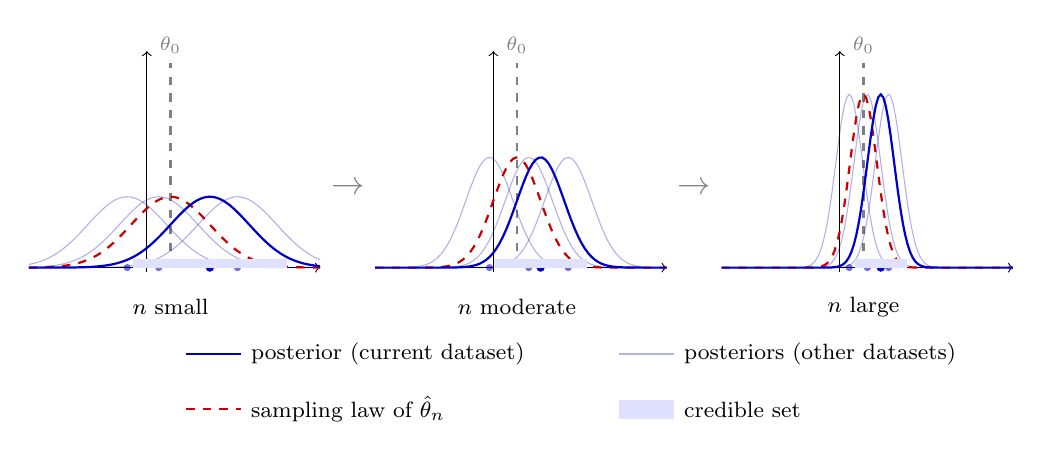
\begin{tikzpicture}
% Raw theta axis. theta_0 = 0.3 (dashed).
% red dashed  : sampling law of hat theta_n, centred at theta_0, width sigma_n.
% blue        : posteriors from several sampled datasets, each width sigma_n,
%               centred at its own random hat theta_n, scattered across the red curve.
% As n grows sigma_n shrinks (all narrow toward theta_0), but the scatter of the
% blue centres always spans the red curve: offset ~ width at every n -> never coincide.

%% Panel 1: n small  (sigma = 0.5)
\begin{scope}[xshift=0cm]
  \draw[->] (-1.5,0) -- (2.2,0);
  \draw[->] (0,-0.05) -- (0,2.75);
  \draw[dashed, gray, thick] (0.3,0) -- (0.3,2.6);
  \node[above, font=\scriptsize, gray] at (0.3,2.6) {$\theta_0$};
  % ensemble of posteriors (faint)
  \foreach \c in {-0.25,0.15,1.15}{
    \draw[blue!70!black, opacity=0.30, domain=-1.5:2.2, samples=90]
      plot (\x,{0.90*exp(-(\x-\c)^2/0.5)});
    \fill[blue!70!black, opacity=0.55] (\c,0) circle (1.3pt);}
  % sampling law (red)
  \draw[red!80!black, dashed, thick, domain=-1.5:2.2, samples=90]
    plot (\x,{0.90*exp(-(\x-0.3)^2/0.5)});
  % representative posterior (solid), centre 0.8
  \draw[blue!80!black, thick, domain=-1.5:2.2, samples=90]
    plot (\x,{0.90*exp(-(\x-0.8)^2/0.5)});
  \fill[blue!80!black] (0.8,0) circle (1.5pt);
  % its 95% credible set: 0.8 ± 1.96*0.5
  \fill[blue!12] (-0.18,0) rectangle (1.78,0.11);
  \node[font=\footnotesize] at (0.3,-0.5) {$n$ small};
\end{scope}

\node[font=\large, gray] at (2.55, 1.0) {$\to$};

%% Panel 2: n moderate  (sigma = 0.3)
\begin{scope}[xshift=4.4cm]
  \draw[->] (-1.5,0) -- (2.2,0);
  \draw[->] (0,-0.05) -- (0,2.75);
  \draw[dashed, gray, thick] (0.3,0) -- (0.3,2.6);
  \node[above, font=\scriptsize, gray] at (0.3,2.6) {$\theta_0$};
  \foreach \c in {-0.05,0.45,0.95}{
    \draw[blue!70!black, opacity=0.30, domain=-1.5:2.2, samples=90]
      plot (\x,{1.40*exp(-(\x-\c)^2/0.18)});
    \fill[blue!70!black, opacity=0.55] (\c,0) circle (1.3pt);}
  \draw[red!80!black, dashed, thick, domain=-1.5:2.2, samples=90]
    plot (\x,{1.40*exp(-(\x-0.3)^2/0.18)});
  \draw[blue!80!black, thick, domain=-1.5:2.2, samples=90]
    plot (\x,{1.40*exp(-(\x-0.6)^2/0.18)});
  \fill[blue!80!black] (0.6,0) circle (1.5pt);
  % 95% credible set: 0.6 ± 1.96*0.3
  \fill[blue!12] (0.012,0) rectangle (1.188,0.11);
  \node[font=\footnotesize] at (0.3,-0.5) {$n$ moderate};
\end{scope}

\node[font=\large, gray] at (6.95, 1.0) {$\to$};

%% Panel 3: n large  (sigma = 0.17) -- peaky, but centres still scattered (NOT coincident)
\begin{scope}[xshift=8.8cm]
  \draw[->] (-1.5,0) -- (2.2,0);
  \draw[->] (0,-0.05) -- (0,2.75);
  \draw[dashed, gray, thick] (0.3,0) -- (0.3,2.6);
  \node[above, font=\scriptsize, gray] at (0.3,2.6) {$\theta_0$};
  \foreach \c in {0.12,0.35,0.62}{
    \draw[blue!70!black, opacity=0.30, domain=-1.5:2.2, samples=120]
      plot (\x,{2.20*exp(-(\x-\c)^2/0.0578)});
    \fill[blue!70!black, opacity=0.55] (\c,0) circle (1.3pt);}
  \draw[red!80!black, dashed, thick, domain=-1.5:2.2, samples=120]
    plot (\x,{2.20*exp(-(\x-0.3)^2/0.0578)});
  \draw[blue!80!black, thick, domain=-1.5:2.2, samples=120]
    plot (\x,{2.20*exp(-(\x-0.52)^2/0.0578)});
  \fill[blue!80!black] (0.52,0) circle (1.5pt);
  % 95% credible set: 0.52 ± 1.96*0.17
  \fill[blue!12] (0.187,0) rectangle (0.853,0.11);
  \node[font=\footnotesize] at (0.3,-0.5) {$n$ large};
\end{scope}

% Legend – 2 × 2 grid
\draw[blue!80!black, thick] (0.5,-1.1) -- (1.2,-1.1);
\node[right, font=\footnotesize] at (1.2,-1.1) {posterior (current dataset)};
\draw[blue!70!black, opacity=0.30, thick] (6.0,-1.1) -- (6.7,-1.1);
\node[right, font=\footnotesize] at (6.7,-1.1) {posteriors (other datasets)};
\draw[red!80!black, dashed, thick] (0.5,-1.8) -- (1.2,-1.8);
\node[right, font=\footnotesize] at (1.2,-1.8) {sampling law of $\hat\theta_n$};
\fill[blue!12] (6.0,-1.92) rectangle (6.7,-1.68);
\node[right, font=\footnotesize] at (6.7,-1.8) {credible set};

\end{tikzpicture}
\caption{The BvM phenomenon as $n$ increases. The red dashed curve is the sampling law of $\hat\theta_n$ (centred at $\theta_0$); blue curves are posteriors from separately sampled datasets, each centred at its own $\hat\theta_n$. As $n$ grows all curves narrow, but each posterior stays centred at $\hat\theta_n$. The posterior width approximately matches the spread of the frequentist sampling distribution, so the $95\%$ credible set (shaded) achieves asymptotically correct frequentist coverage.}
\label{fig: BvM schematic}
\end{figure}

These two objects answer different questions: one describes what would happen across many hypothetical experiments, the other describes uncertainty given the single observed dataset. Crucially, a $95\%$ credible set $C_n$ satisfies $\Pi(\theta \in C_n \mid Z_1,\ldots,Z_n) \geq 0.95$ by definition, but there is no guarantee that it will contain the underlying true parameter $\theta_0$. In parametric models, however, the BvM theorem guarantees that the posterior converges in total variation to the same limiting Gaussian as the sampling distribution of $\hat\theta_n$, so a $(1-\alpha)$ credible set is asymptotically a valid $(1-\alpha)$ frequentist confidence set.



\paragraph{Why UQ is harder in nonparametric inverse problems.}
In nonparametric inverse problems the situation is fundamentally harder, for two reasons. First, the rates of convergence are non-standard: in Wicksell's problem the optimal rate for estimating $F_0(x)$ is $\sqrt{n}/\sqrt{\log n}$, slower than $\sqrt{n}$ by a logarithmic factor, so the rescaling in the BvM display above is no longer $\sqrt{n}$. Second, the limiting distributions involve nuisance parameters, like the local density $g_0(x)$ and the local H\"{o}lder smoothness $\gamma$ of $F_0$, that are themselves difficult to estimate consistently. For a frequentist, constructing a confidence interval therefore requires estimating these nuisance quantities, which introduces additional uncertainty and may lead to under-coverage in practice. Bootstrap procedures are an attractive alternative; while they can fail in non-standard-rate settings \cite{63}, a consistent bootstrap does exist for Wicksell's problem.

The Bayesian approach offers a way out. One places a nonparametric prior $\Pi$ on $F_0$ and studies the posterior $\Pi(\,\cdot\mid Z_1,\ldots,Z_n)$. Credible sets are produced automatically as a by-product of posterior computation and do not require the user to estimate nuisance parameters. Whether these credible sets are valid from a frequentist perspective depends on whether a nonparametric analogue of the BvM theorem holds. The rigorous justification is provided by \textit{semiparametric BvM theorems}: under suitable conditions, the posterior for a functional $T(F_0)$, after centring at an efficient estimator and rescaling at the correct rate, converges to the same Gaussian as the sampling distribution of that estimator. While such results require considerably more work than in the parametric case \cite{208}, in the inverse-problem settings treated in this thesis, a BvM theorem takes the form: there exists an efficient estimator $\hat{T}_n$ and a variance $\sigma^2$ such that
\[
\sup_{B}\left|\Pi\!\left(r_{n}\,( T(F) - \hat{T}_n) \in B \;\big|\; Z_1,\ldots,Z_n\right) - \Phi_{\sigma^2}(B)\right| \xrightarrow{\pb_{F_0}} 0,
\]
where $r_n$ is a rate, $\Phi_{\sigma^2}$ is the centred Gaussian with variance $\sigma^2$ and the supremum is over Borel sets $B$. The variance $\sigma^2$ is the asymptotic variance of the efficient estimator and does not involve nuisance parameters beyond those already determined by $F_0$ itself. Figure~\ref{fig: BvM schematic} illustrates schematically how the BvM theorem aligns the posterior with the frequentist sampling distribution, making Bayesian credible sets into asymptotically valid frequentist confidence sets.

\section{How is this thesis built?}\label{par: outline}
The organisation of the this is as follows.

\medskip
\noindent\textbf{Chapter~2 --- Frequentist nonparametric estimation in Wicksell's problem.}
Wicksell's problem originates in the medical setting: it was introduced to model the size distribution of spherical tumours in the spleen from post-mortem cross-sections. More generally, in materials science and stereology \cite{14} we have the following setting: spherical particles of unknown radii are embedded in an opaque medium, and the only observable data are the radii of the circles produced when a plane cuts through the medium. Very interestingly, the same underlying mathematical structure appears in astronomy \cite{33, 19}: one observes only the two-dimensional projected positions of stars in a globular cluster and wishes to recover the three-dimensional radial distribution. In both settings, the forward operator maps the distribution $F_0$ of squared sphere radii to the distribution $G_0$ of squared circle radii through an Abel-type integral equation, and the inversion formula involves the functional $V_0(x) = \int_x^\infty g_0(z)(z-x)^{-1/2}\,dz$. The nonparametric estimation of $F_0$ in this setting was pioneered by Groeneboom and Jongbloed \cite{1}, who established rates of convergence for an isotonic estimator; the question of asymptotic efficiency was subsequently studied by Golubev and Levit \cite{10}, who identified the optimal asymptotic variance. The naive empirical plug-in estimator of $V_0$ is non-monotone and erratic; its isotonised version, the \textit{isotonic inverse estimator} (IIE), is monotone by construction. Chapter~2 establishes that the IIE adapts automatically to the \textit{local} H\"{o}lder smoothness $\gamma > 1/2$ of $F_0$ at the estimation point and at zero, without requiring knowledge of $\gamma$, and that it attains the minimax lower bound, making it the uniquely efficient nonparametric estimator in this problem. A striking consequence is that when $F_0$ is flat near the estimation point, the IIE automatically attains the faster $\sqrt{n}$ rate --- a phenomenon with no analogue in standard nonparametric density estimation.

\medskip
\noindent\textbf{Chapter~3 --- Bayesian nonparametric approaches to Wicksell's problem.}
In this chapter, we develop two distinct Bayesian nonparametric approaches to Wicksell's problem. The first, and main, approach places a Dirichlet Process prior directly on the \textit{observable} distribution $G_0$, which is conjugate and computationally explicit. The key innovation is to isotonise the posterior draws, projecting each draw through the inversion and isotonisation pipeline, to obtain the \textit{Isotonized Inverse Posterior} (IIP), following the projection-posterior methodology of Chakraborty and Ghosal \cite{60,54}. The main results are semiparametric BvM theorems: the IIP concentrates at the optimal rate $\sqrt{n}/\sqrt{\log n}$ with a variance that adapts to the local smoothness $\gamma > 1/2$, without estimating any nuisance parameter, and the resulting credible sets have asymptotically correct frequentist coverage. These results were published in the \textit{Annals of Statistics} \cite{51}. The second approach places a Dirichlet Process prior directly on \textit{the unknown} $F_0$ itself, yielding a hierarchical Dirichlet-Beta model. Here the posterior is a mixture of Dirichlet processes, and a BvM theorem is currently out of reach; instead, posterior consistency and contraction rates are established for this more classical Bayesian formulation.

\medskip
\noindent\textbf{Chapter~4 --- Semiparametric UQ via isotonized posterior for deconvolutions.}
The deconvolution problem on the half-line arises when one observes $Z_i = X_i + Y_i$, where $0 \le X_i \sim F_0$ is the unknown quantity of interest and $Y_i$ follows a known distribution with density $k$ on $[0,\infty)$. Applications include back-calculation of historical HIV infection rates in epidemiology \cite{61}, image restoration \cite{68,67}, astronomical spectroscopy, and seismology. Chapter~4 develops the isotonized-posterior methodology for this setting. A Dirichlet Process prior is placed on the observable distribution $G_0$ and the posterior draws are isotonised, producing the IIP $\hat{F}_{\scriptscriptstyle{G}}$. The main result is an analogue of the asymptotic distribution theorem of van~Es, Jongbloed, and van~Zuijlen \cite{74} for the Bayesian procedure: $n^{1/3}(\hat{F}_{\scriptscriptstyle{G}}(x) - F_0(x))$ converges, conditionally on the data, to the \textit{Bayesian Chernoff distribution} introduced by Chakraborty and Ghosal \cite{54} --- the same distribution that governs isotonic regression posteriors. This parallels exactly the cube-root Chernoff asymptotics of the frequentist IIE, establishing a precise frequentist-Bayesian correspondence in a non-Gaussian, non-$\sqrt{n}$ regime. Because the limiting distribution is non-Gaussian, classical BvM theory does not apply; valid credible sets require a known recalibration of the type developed by Chakraborty and Ghosal in \cite{54}, and the question of efficiency in any rigorous sense remains open.

\medskip
\noindent\textbf{Chapter~5 --- Proximal causal inference via mixtures of linear models.}
The final chapter addresses causal inference in the presence of unmeasured confounding, a challenge that arises in observational studies in medicine, economics, and the social sciences. When treatment and outcome are both affected by a latent confounder $U$, standard regression does not recover the causal effect. \textit{Proximal inference} \cite{205,120} provides a solution by exploiting proxy variables: a negative-control exposure $Z$ (not causing the outcome $Y$) and a negative-control outcome $W$ (not causally affected by treatment $A$). Under suitable completeness conditions, the average causal effect of $A$ on $Y$ is identifiable from the observed distribution of $(A,W,Y,Z)$ via a \textit{bridge function}. Existing identification results rely on strong linearity or categoricity assumptions. Chapter~5 introduces a causal model based on mixtures of linear models for the regression of $Y$ on the unmeasured confounder, a strategy also adopted concurrently and independently in the related work of Hu, Zorzetto, and Dominici \cite{209}. Under this model the bridge function exists and has a closed-form expression, extending identifiability to a substantially richer class of outcome models. A Bayesian nonparametric estimator is proposed, based on a probit stick-breaking process with covariate-dependent mixing weights, and a posterior consistency theorem for the average treatment effect is proved by establishing Kullback-Leibler support and sieve entropy conditions for the dependent mixture prior.

\paragraph{In an ideal world: a programme for efficiency and UQ.}
The ideal approach to each inverse problem would follow five steps.
\begin{enumerate}[leftmargin=*, label=(\roman*)]
  \item \textbf{Construct a shape-constrained frequentist estimator.} Compose the empirical plug-in with an isotonisation or regularisation step to obtain a monotone, tuning-parameter-free estimator of the functional of interest.
  \item \textbf{Derive the limiting distribution.} Establish that the estimator, after appropriate centring and rescaling by a rate $r_n$, converges in distribution to a known limit law. In the Gaussian case this yields an asymptotic variance $\sigma^2(F_0)$ that may depend on local properties of $F_0$ --- such as the local H\"{o}lder smoothness $\gamma$ or the density $g_0(x)$ --- but the estimator should adapt to these automatically, without knowing $\gamma$ or $g_0$.
  \item \textbf{Prove a matching minimax lower bound.} Show that no estimator sequence can have a smaller asymptotic mean squared error than $r_n^{-2}\,\sigma^2(F_0)$, uniformly over a suitable class $\mathcal{F}$. Together with step~(ii), this certifies the estimator as asymptotically efficient: it is the best possible in both rate and constant.
  \item \textbf{Construct a Bayesian counterpart.} Place a nonparametric prior on the observable distribution $G_0$ and apply the same isotonisation pipeline to the posterior draws, obtaining an \textit{Isotonized Inverse Posterior} (IIP) that is computationally no harder than the frequentist estimator.
  \item \textbf{Prove a Bernstein-von Mises theorem.} Show that the IIP concentrates at the same rate $r_n$ and with the same variance $\sigma^2(F_0)$ as the efficient frequentist estimator. By step~(iii), the posterior is then \textit{Bayes-efficient}: its $(1-\alpha)$ credible sets are asymptotically valid $(1-\alpha)$ frequentist confidence sets at the minimax-optimal level, free of nuisance parameters.
\end{enumerate}
Unfortunately we do not live in an ideal world and bringing this program to completion is a considerable undertaking that not always is possible, also because some mathematical concepts are not yet clear (!), e.g.\ the concept of efficiency for non-Gaussian limiting distributions.

\smallskip
\noindent\textit{Wicksell's problem (Chapters~2--3).}
This is the setting where the complete chain is established. Chapter~2 constructs the IIE, derives its limiting distribution, and proves the matching minimax lower bound, establishing the IIE as asymptotically efficient. Chapter~3 then constructs the Bayesian counterpart (the IIP) and proves a semiparametric BvM theorem showing that the posterior concentrates with the same asymptotic variance, making the credible sets asymptotically valid confidence sets at the minimax-optimal level. 

\smallskip
\noindent\textit{Deconvolution (Chapter~4).}
For the deconvolution problem on the half-line, the situation is different. The asymptotic distribution of the isotonic inverse estimator was already established by van~Es, Jongbloed, and van~Zuijlen \cite{74}, so step~(ii) of the programme was known prior to this thesis. Crucially, however, the limiting distributions in the deconvolution setting are in general \textit{not Gaussian}: depending on the kernel and the smoothness of $F_0$, one encounters non-standard limit laws. This means that the standard theory of semiparametric efficiency --- which is built around Gaussian limits and Fisher information --- does not directly apply, and the question of whether the IIE is efficient in any rigorous sense remains open in the literature. The contribution of this thesis, developed in Chapter~4, is to show that the Bayesian IIP behaves asymptotically in the same way as the frequentist IIE. The two procedures do not agree exactly in distribution: the posterior requires a known calibration in order for its credible sets to achieve correct frequentist coverage, of the type studied by Chakraborty and Ghosal in the related monotone regression setting \cite{54,60}. Steps~(iii) (minimax lower bound matching the Bayesian variance) and a full treatment of efficiency thus remain open.

\smallskip
\noindent\textit{Causal inference (Chapter~5).}
Proximal causal inference is a relatively nascent field, and many fundamental questions like identification conditions, optimal estimation rates and efficiency bounds remain unsettled in the literature \cite{205,120}. Chapter~5 takes a more modest first step: it introduces a flexible causal model based on mixtures of linear models, establishes identifiability of the average treatment effect in closed form, proposes a Bayesian nonparametric estimator, and proves that this estimator is consistent. The questions of efficient estimation, asymptotic distributions, and UQ in the proximal causal setting are, to the best of my knowledge, still to these days open problems.

\paragraph{Scope of this thesis.}\label{par: aim}
The common thread of this thesis is the study of Bayesian nonparametric procedures for statistical inverse problems. For each problem considered, we design a procedure, typically by placing a nonparametric prior on the observable distribution and isotonising the posterior draws, and then investigate its theoretical properties: posterior consistency, asymptotic distribution, and the validity of the resulting uncertainty quantification. Where possible, we compare the Bayesian procedure to its frequentist counterpart and ask whether the two are asymptotically equivalent; where a notion of efficiency is available, we ask whether the procedure is optimal. The answers vary by problem. For Wicksell's problem the analysis can be carried to completion: we obtain an efficient frequentist estimator, a matching minimax lower bound, and a Bayesian procedure that is asymptotically equivalent to the efficient estimator, giving valid and nuisance-parameter-free credible sets. For deconvolution, the Bayesian procedure can be shown to match the frequentist one asymptotically, but efficiency in the classical sense is not defined because the limiting distributions are non-Gaussian. For the causal inference problem, consistency of the Bayesian estimator is the main result, and the deeper questions of asymptotic distribution and efficiency are left open. 